\thispagestyle{fancy}
\vspace*{40 pt}
\subsection{Tela comando slotter}\label{telaComandoSlotter}
 Esta tela é acessada pelo botão "\textgreater" no menu superior esquerdo da tela de comando da ultima impressora, pelo botão "\textless{}" no menu superior esquerdo da tela comando perfuradora, pelo botão "SLT" em qualquer tela de comando e pelo botão comando da tela ajustes slotter.
 \vspace*{\fill}
 \begin{figure}[h]
  \centering
  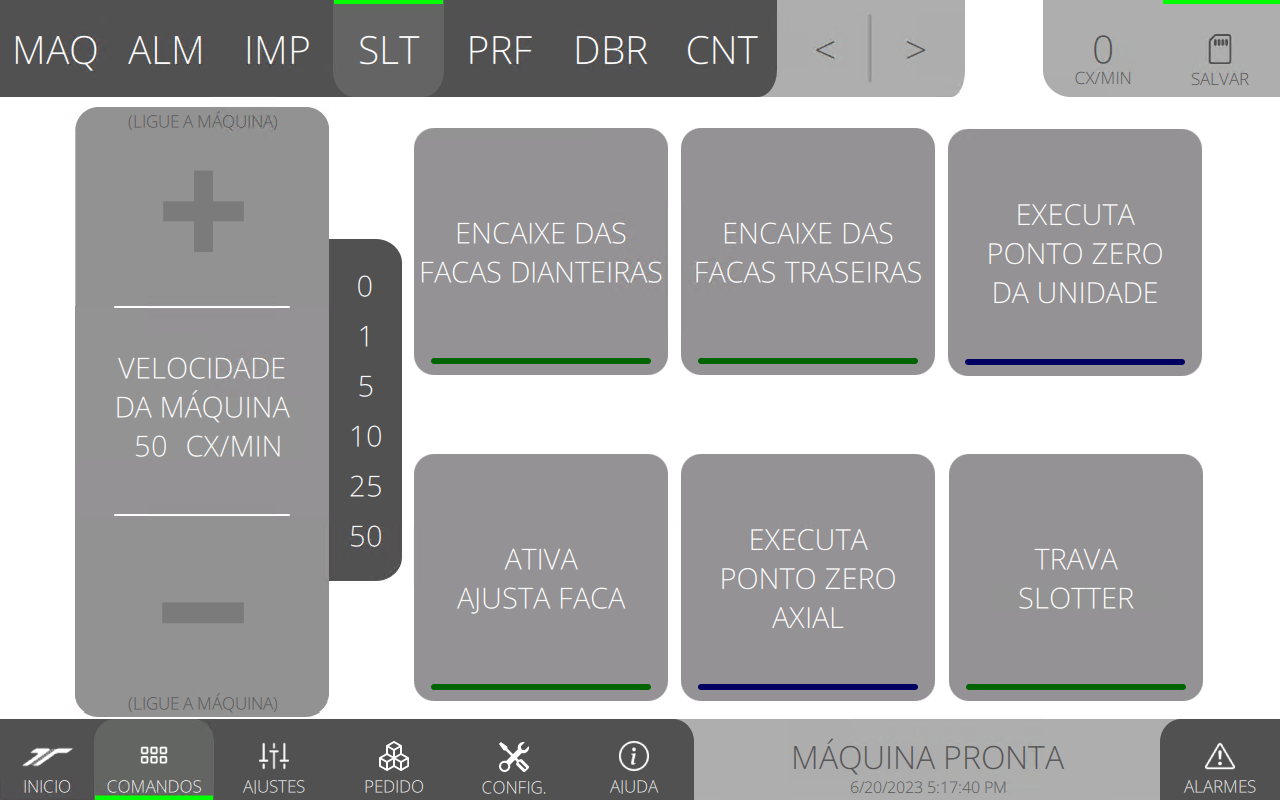
\includegraphics[width=576px,height=360px]{src/imagesMiniline/05-Slotter/Commands/e0.png}
\end{figure}
\vspace*{\fill}

\newpage
\thispagestyle{fancy}
\vspace*{40 pt}
\subsubsection{\small{Encaixe das facas traseiras}}\label{telaComandoSlotterEncaixeDasFacasTraseiras}
\vspace*{\fill}
\begin{figure}[h]
  \centering
  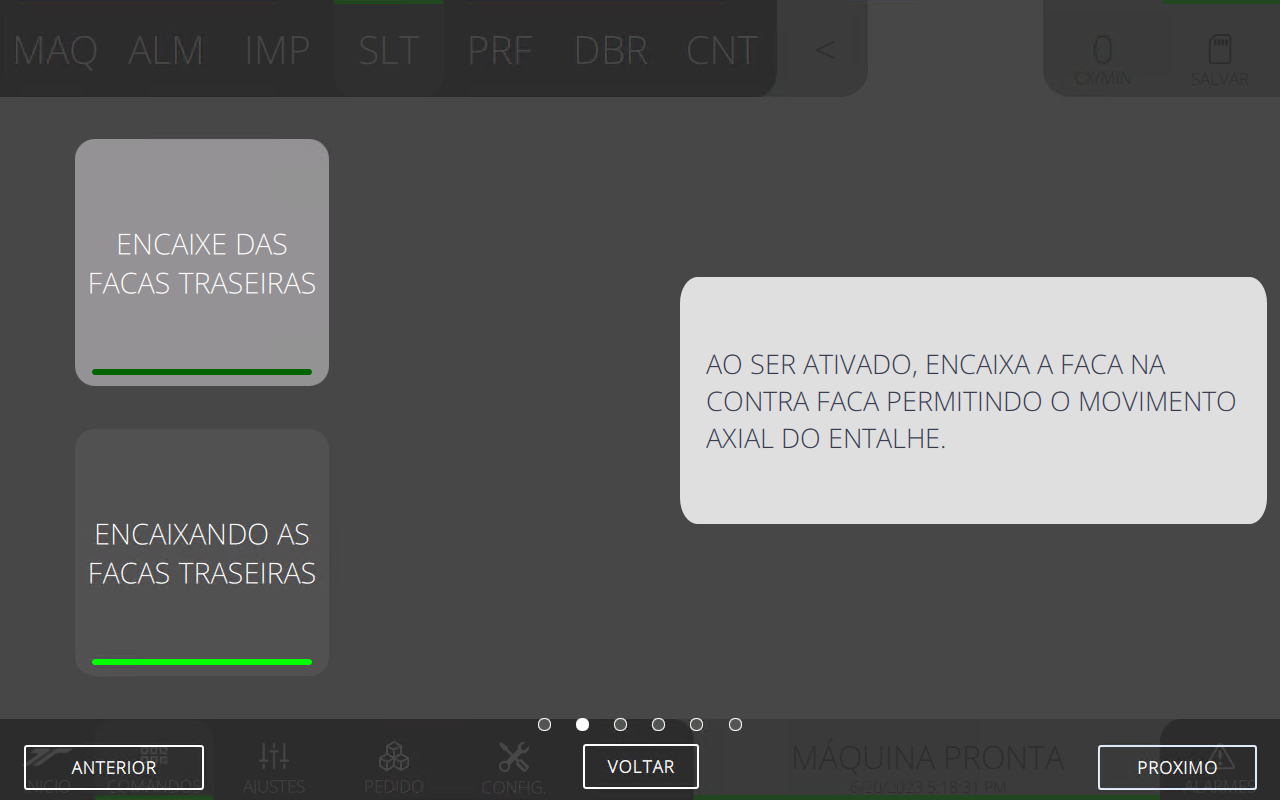
\includegraphics[width=576px,height=360px]{src/imagesMiniline/05-Slotter/Commands/e2.png}
\end{figure}
\vspace*{\fill}

\newpage
\thispagestyle{fancy}
\vspace*{40 pt}
\subsubsection{\small{Executa ponto zero da unidade}}\label{telaComandoSlotterExecutaPontoZeroDaUnidade}
\vspace*{\fill}
\begin{figure}[h]
  \centering
  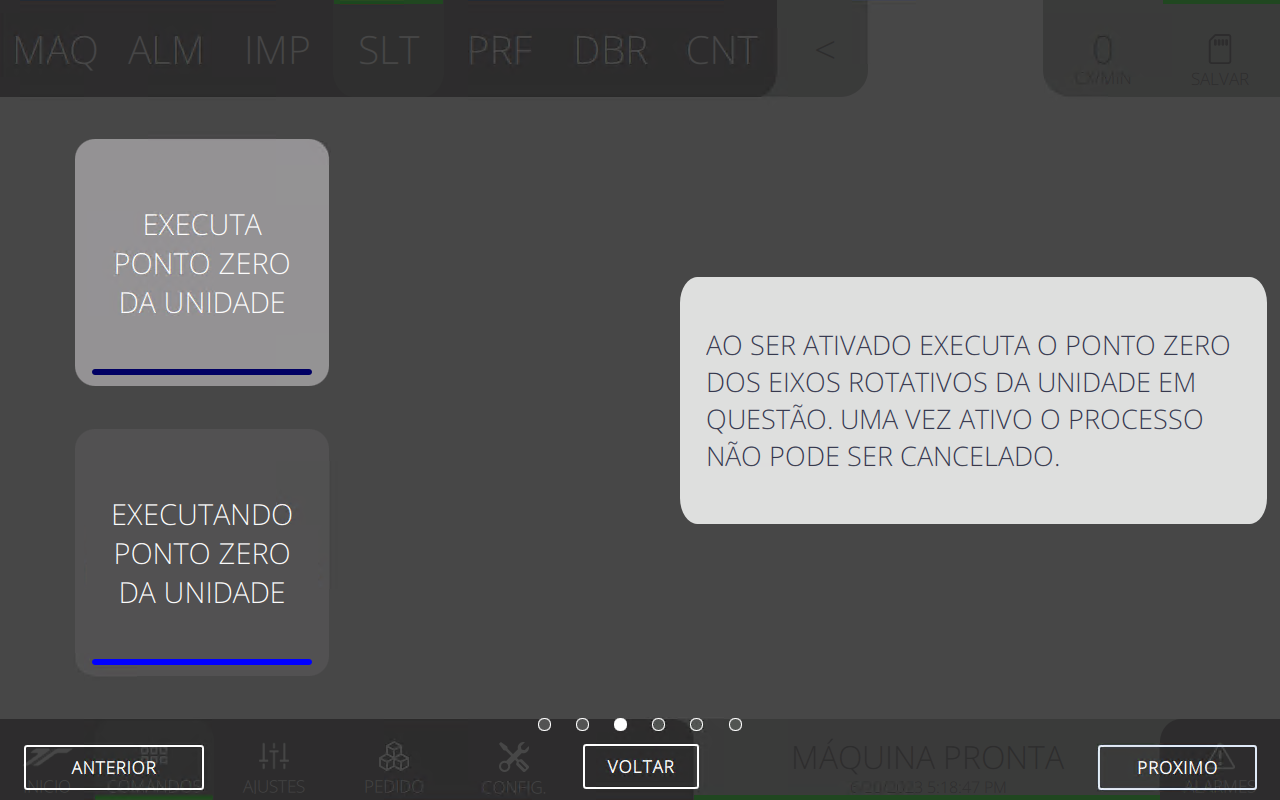
\includegraphics[width=576px,height=360px]{src/imagesMiniline/05-Slotter/Commands/e3.png}
\end{figure}
\vspace*{\fill}


\newpage
\thispagestyle{fancy}
\vspace*{40 pt}
\subsubsection{\small{Executa ponto zero axial}}\label{telaComandoSlotterExecutaPontoZeroAxial}
\vspace*{\fill}
\begin{figure}[h]
  \centering
  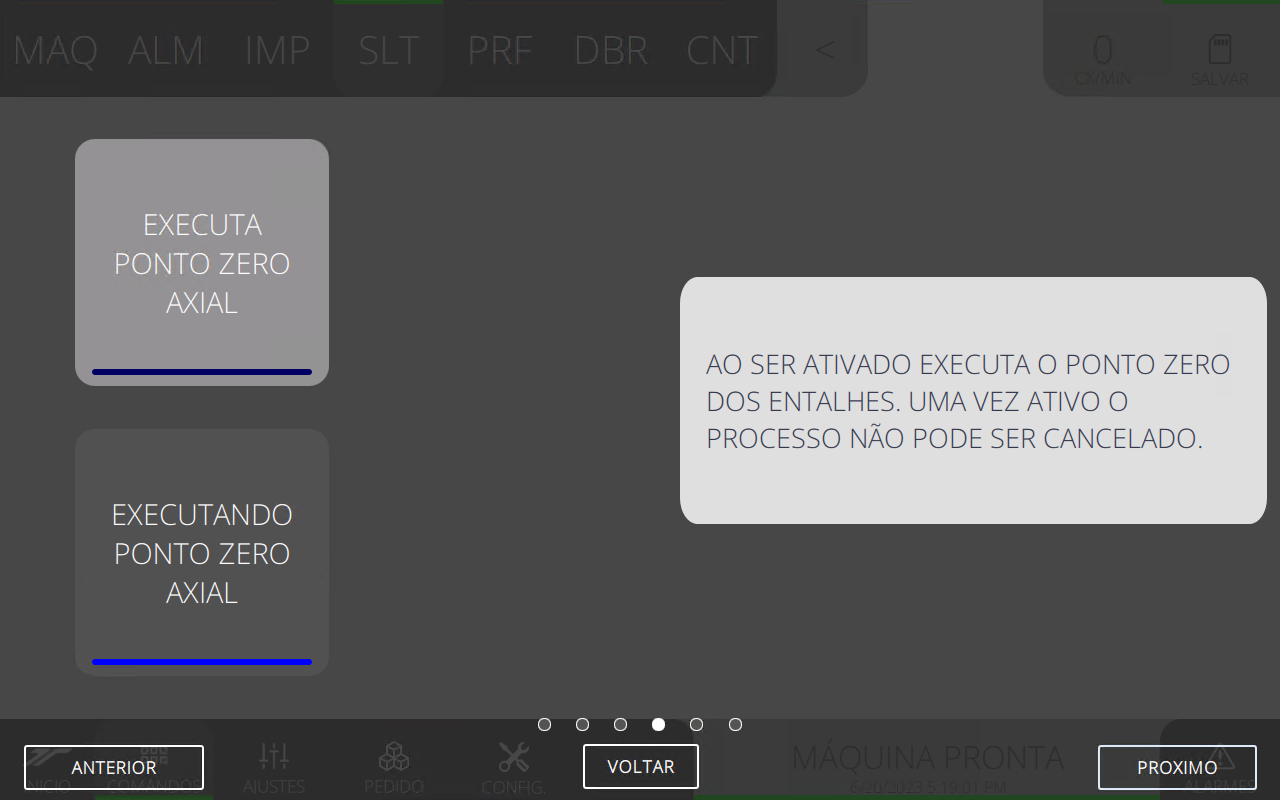
\includegraphics[width=576px,height=360px]{src/imagesMiniline/05-Slotter/Commands/e4.png}
\end{figure}
\vspace*{\fill}

\newpage
\thispagestyle{fancy}
\vspace*{40 pt}
\subsubsection{\small{Encaixe das facas dianteiras}}\label{telaComandoSlotterEncaixeDasFacasDianteiras}
\vspace*{\fill}
\begin{figure}[h]
  \centering
  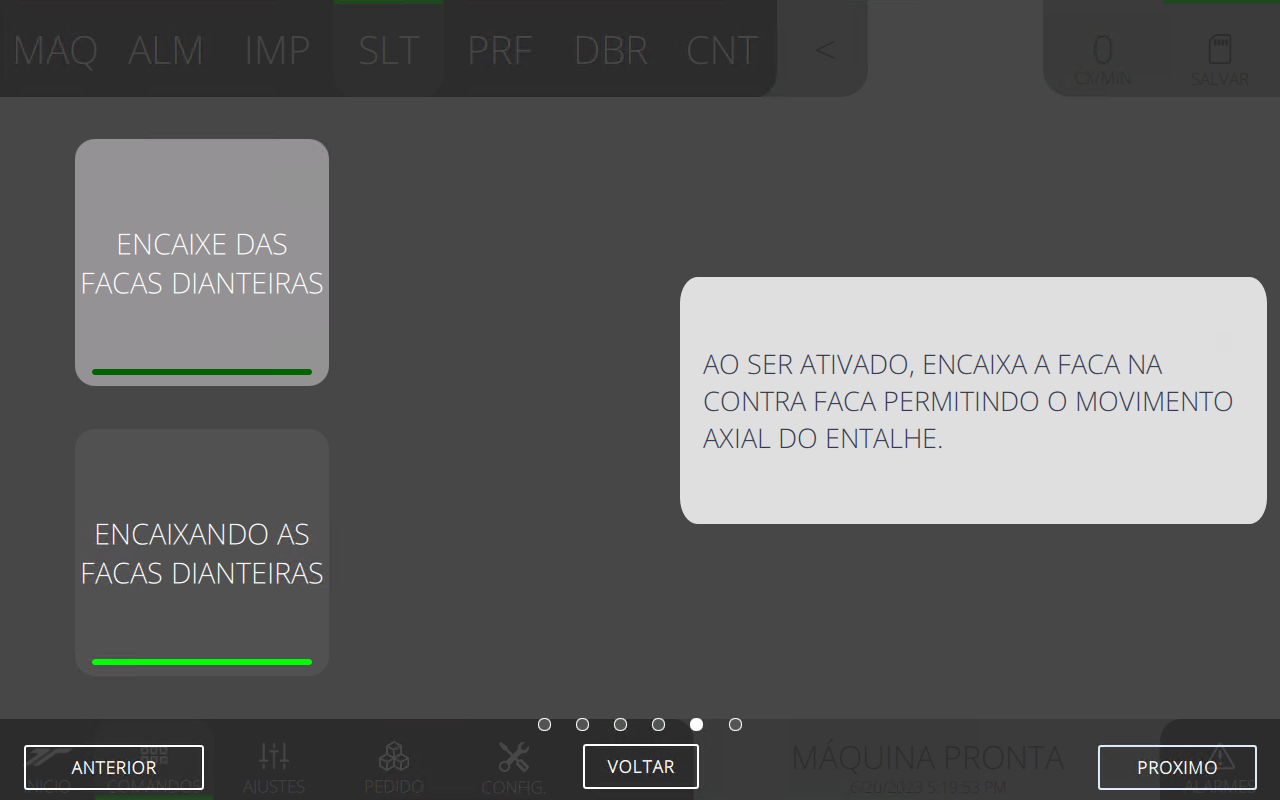
\includegraphics[width=576px,height=360px]{src/imagesMiniline/05-Slotter/Commands/e5.png}
\end{figure}
\vspace*{\fill}

\newpage
\thispagestyle{fancy}
\vspace*{40 pt}
\subsubsection{\small{Comando trava slotter}}\label{telaComandoSlotterComandoTravaSlotter}
\vspace*{\fill}
\begin{figure}[h]
  \centering
  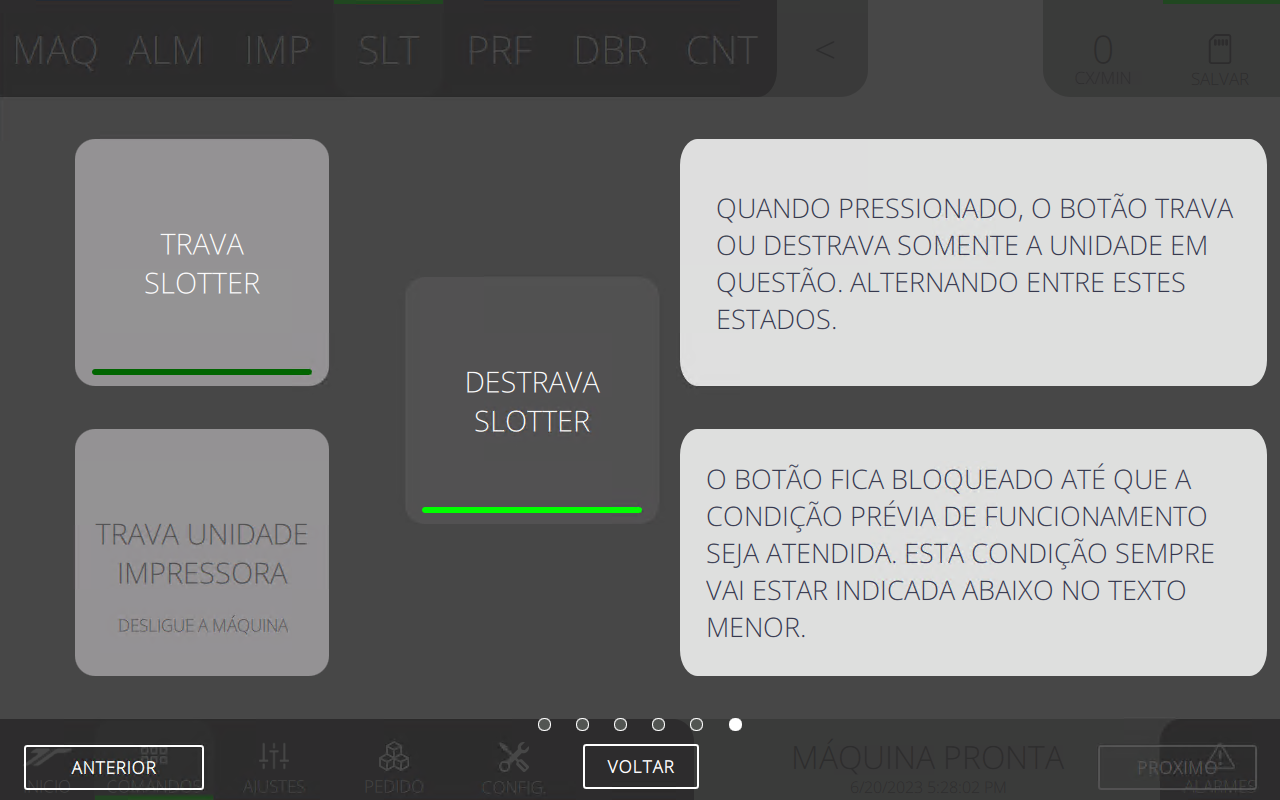
\includegraphics[width=576px,height=360px]{src/imagesMiniline/05-Slotter/Commands/e6.png}
\end{figure}
\vspace*{\fill}

\newpage
\thispagestyle{fancy}
\vspace*{40 pt}
\subsubsection{\small{Comando ajusta faca}}\label{telaComandoSlotterComandoAjustaFaca}
\vspace*{\fill}
\begin{figure}[h]
  \centering
  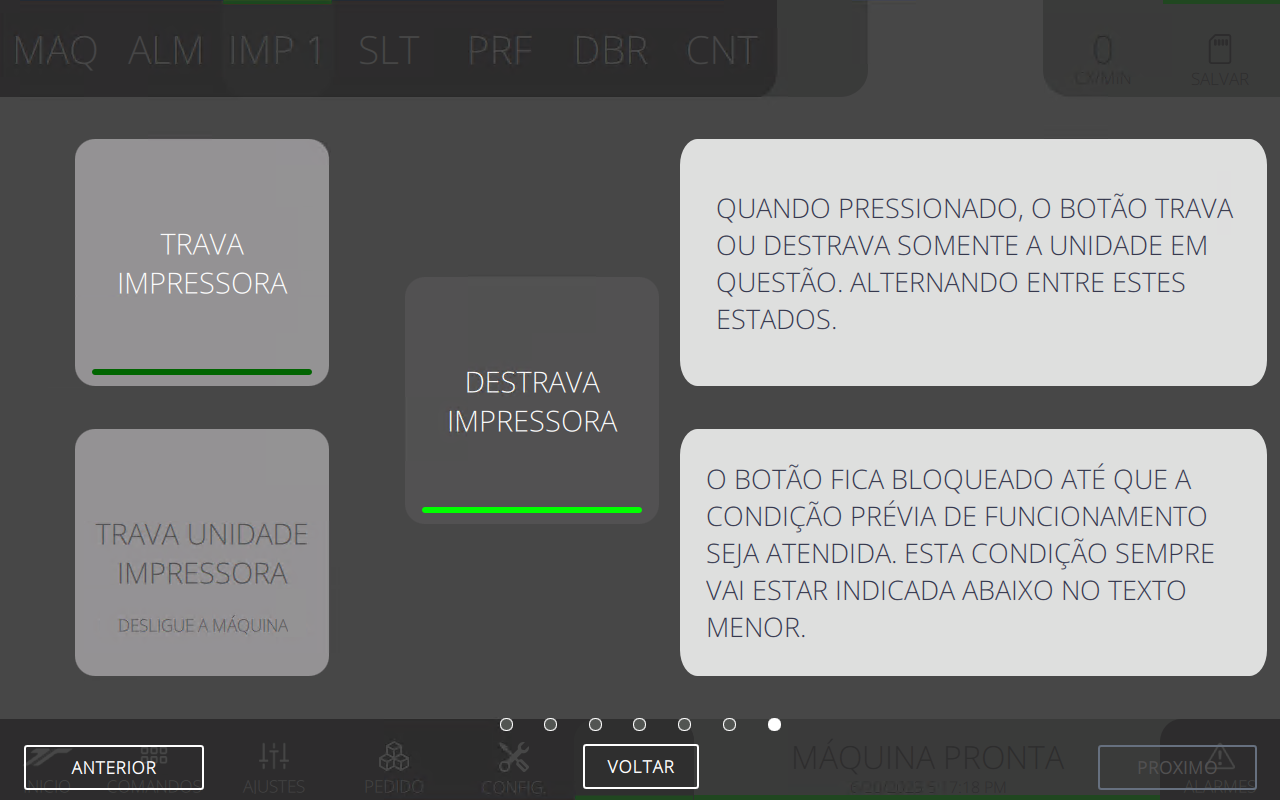
\includegraphics[width=576px,height=360px]{src/imagesMiniline/05-Slotter/Commands/e7.png}
\end{figure}
\vspace*{\fill}

